\chapter{Background}

\section{Early-Type Stars}
\label{sec:earlytype}

%//TODO I quite like this joke but it needs a bit of work
The term Early-type stars is quite possibly the epitome of bad naming conventions in astrophysics, it's a very old term, coming from the dawn of astrophysics itself, quite opaque as to what it means, and also by definition \textit{completely wrong}. In fact it is one of the most wrong pieces of terminology I can think of.\footnote{Aside from astrophysicists calling something ``warm'', of course. That can quite literally mean anything from 10 to 10,000 Kelvin, depending on who you ask, what they're writing about, or how they're feeling at that particular moment. In fact, I'll probably end up falling into this same trap somewhere in this thesis as well!}
The first generation of astrophysicists found themselves asking very important questions such as ``what even \textit{are} stars?'' and ``what possible mechanism can allow a star to burn for so long?'' Each of these questions was rather pressing for the burgeoning field, and the scientific community was aching for an answer.

Of course, like all pressing questions of the \nth{19} century, it fell to Lord Kelvin to provide a convincing but incorrect answer. Kelvin assumed that gravitational collapse was the mechanism for a stars long-term heating, with younger, ``early'' type stars shining the brightest. Not only was the mechanism incorrect, but typically older main sequence stars are more luminous than their younger counterparts of a similar mass! However, as is the case with astrophysical terminology, the term stuck, to the confusion of many young astrophysicists.

%//FIXME POTENTIAL maybe put this part in with OB stars? allows for more seamless switching from diatribe to the main body

Instead, we now know that stars produce their energy through fusion. These reactions vary from sub-stellar deuterium and lithium burning, to main sequence p-p \& CNO hydrogen burning processes, and finally to the triple-$\alpha$ and other exotic fusion processes for evolved massive stars. The more massive the star the greater the internal pressure, allowing for more exotic fusion processes.
The bigger a star, the greater the core pressure and temperature, as all fusion reactions are highly dependent on temperature, stars with only a few dozen solar masses are thousands of times more luminous than our sun, but only live a fraction of the time \parencite{carrollIntroductionModernAstrophysics2014}.

\subsection{OB-type stars}
\label{sec:obtype}

And with that we shift our gaze to high-mass stars, with the most massive of all being the O and B type stars, these are extremely luminous ($\sim 10^4 \,\si{\solarluminosity}$), and relatively short lived ($\sim 10 \, \si{\mega\year}$) stars. The age-old adage of a candle burning twice as bright lasting half as long applies to our studies of the cosmos, but it is more apt to compare a candle and a stick of dynamite when considering stars on opposing ends of the Harvard classification system.

% Formation of OB stars, note binary systems!

The most common formation mechanism of stars is through the collapse of a giant molecular cloud\footnote{GMC}, an enormous cool cloud many parsecs across with a mass of around $10^4 \si{\solarmass}$.
As this GMC collapses and radiates energy, lowering the radius of thermostatic equilibrium for the cloud, as collapsing progresses the cloud fragments into many smaller regions with a critical density, capable of collapsing further, forming a star.
The collapse of a GMC can be described with a series of timescale.
First, the Kelvin-Helmholtz timescale, $\tau_{KH}$, which describes the timescale required for the radiating cloud to collapse.
The second important timescale is the free-fall timescale, $\tau_{ff}$, which is the time taken for a cloud to collapse. These timescales are described by the following equations:

\begin{subequations}
  \begin{align}
      \tau_{KH} & \approx \frac{GM_*^2}{R_*L_*} \label{eq:khtime} ,\\
      \tau_{ff} & = \sqrt{\frac{3\pi}{32G\bar{\rho}}} \label{eq:fftime} ,
  \end{align}
  \label{eq:khfreefalltimes}
\end{subequations}

where $M_*$ is the protostellar mass, $R_*$ is the protostellar radius, $L_*$ is the protostellar luminosity, and $\rho$ is the mean density of the collapsing cloud \parencite{ward-thompsonIntroductionStarFormation2011}.

%//TODO is the above section completely necessary? it might be better to just describe star formation.

Perhaps the most important distinction between massive star formation and its better understood counterpart is as a young protostar approaches the main sequence, the KH timescale is less than the free-fall timescale, meaning the material at the center of the collapsing cloud begins fusion while the bulk of core has collapsed onto the site of the future star. This burgeoning star begins to drive the weakly gravitationally coupled collapsing material away due to its sheer luminosity, driving this material outwards, causing it to accrete and shock material within the GMC. 

Another important consideration is the role of angular momentum as the star collapses.
The particularly massive cloud involved in massive star formation is more prone to fragmentation, meaning that massive stars typically form with an orbital partner, whilst approximately 2/3\textsuperscript{rds} of low-mass stars are part of a binary or multiple system, this value is near-total.
As such, the environment within an OB association after star formation consists of numerous young stars in tightly-knit groups disrupting the entire local area.\footnote{This is a bit like living in Headingley, Hyde Park, or any other area with lots of Undergraduates.}

%//TODO cite "near total" statistic, it's in one of the more recent papers you've had a look at, maybe a williams one?

Above a stellar mass of $1.3 \si{\solarmass}$ pressures and temperatures within a stellar core favour the fusion of hydrogen into helium through the catalytic CNO cycle, instead of the more direct p-p fusion process. 

\begin{subequations}
  \begin{align*}
    \prescript{12}{6}{C} + \prescript{1}{1}{H} & \rightarrow \prescript{13}{7}{N} + \gamma \\ 
    \prescript{13}{7}{N} & \rightarrow \prescript{13}{6}{C} + e^+ + \nu_e \\
    \prescript{13}{6}{C} + \prescript{1}{1}{H} & \rightarrow \prescript{14}{7}{N} + \gamma \\
    \prescript{14}{7}{N} + \prescript{1}{1}{H} & \rightarrow \prescript{15}{8}{O} + \gamma \\
    \prescript{15}{8}{O} & \rightarrow \prescript{15}{7}{N} + e^+ + \nu_e \\
    \prescript{15}{7}{N} + \prescript{1}{1}{H} & \rightarrow \prescript{12}{6}{C} + \prescript{4}{2}{He} 
  \end{align*}
\end{subequations}
%//FIXME sort out italics, use regular fonts
%//TODO add net energy gains losseslosses
%//TODO Check to see if this is correct


%//FIXME mechanism less efficient, 0.6MeV per nucleon, but reaction rate just quite a lot faster, temperature sensitivity, series of power laws, t^40 for 1e8k and t^20 for 2e8k
The reaction rate of CNO rises much faster, resulting in a convective core, surrounded by a radiative envelope \parencite{salarisEvolutionStarsStellar2005}. This is the driving force behind the incredible luminosities of an OB star as it hurtles along the main sequence.

%//TODO might be a good idea to include that one graph with fusion rates?

% Influence of OB stars on surrounding environment, outsized influence etc.

% Touch on stellar winds, expand in next section

% Evolution and fate of massive stars, evolution, depletion of hydrogen products, then onto helium burning

Unfortunately for massive stars, pesky fundamental laws such as the conservation of energy come into play. With only an order of magnitude or two of additional mass more than our sun and shining $10^4$ times as brightly, this curtails the life of the brightest stars to lifespans not much more than $10^7$ years.
If we define a galactic year as the time it takes for a star to orbit the Milky Way, these poor stars don't even make it to their first birthdays, which is quite sad really.\footnote{Continuing this analogy our sun can drink, might have voted if they felt like it, and may be racking up vast quantities of student debt.}


As the available hydrogen begins to become depleted, the lowering reaction rates force the star to shrink, this raises the internal temperature until the core begins to burn helium through the triple-$\alpha$ process:

\begin{subequations}
  \begin{align*}
    \prescript{4}{2}{\text{He}} + \prescript{4}{2}{\text{He}} & \rightarrow \prescript{8}{4}{\text{Be}} \\
    \prescript{8}{4}{\text{Be}} + \prescript{4}{2}{\text{He}} & \rightarrow \prescript{12}{6}{\text{C}} + 2\gamma
  \end{align*}
\end{subequations}

The sudden spike in energy radiating from the core shifts the calculus of hydrostatic equilibrium in the favour of outward forces, causing the star to rapidly expand in the form of a Red Supergiant or Luminous Blue Variable \parencite{ryanStellarEvolutionNucleosynthesis2010a}.
During this phase the energy output of the star is even greater, with a timescale of $\sim 10^6$ years, this is only temporarily prolonging the life of the star, which will inevitably begin burning heavier and heavier elements, faster and faster.
Once the star starts producing iron its fate is sealed, the star stops fusing, and collapses, annihilating itself in the form of a supernova and leaving behind a remnant of its core in the form of a neutron star or black hole 
\parencite{ward-thompsonIntroductionStarFormation2011}.

Whilst the stars end is as inevitable as it is violent, the intermediate stage as the star leaves the main sequence is in itself extremely interesting, and for the context of this thesis, no product of this stage is more interesting than the Wolf-Rayet.



\subsection{Wolf-Rayet stars}
\label{sec:wrtype}


%Notes: Evolution type 
% Jumping off point, wiki wolf-rayet current models, research papers therein
% For WC formation O->RSG->WNE->WC 20-45 msol
% WR in general O->LBV->WR

% History and background of Wolf-Rayet stars

% Description of Wolf-Rayet star, introducing concept of strong stellar wind

As we now know, Wolf-Rayets\footnote{Abbreviated to WR.} are evolved forms of O-type stars, and are a short lived component of the life-cycle of massive stars, typically lasting for around \num{5e5} years \parencite{crowther_physical_2007}.
Despite this relatively transient length of this stage, the influence of a WR star on its local medium is extremely outsized.
WR stars in particular are known for having dense, fast winds, typically between 2 and 3 orders of magnitude than their main sequence O-type progenitors, with mass loss rates on the order of $10^{-5} \, \si{\solarmass\per\year}$ and wind velocities of $\num{1.5e3} \, \si{\kilo\metre\per\second}$.
This extremely dense wind is driven by the highly energetic helium burning core, which is luminous enough as to drive away the outer layers of the stars envelope, exposing the core.
The observed spectroscopic lines are due to heating of the envelope from the core, which is enriched with by-products of hydrogen and helium burning, the lack of hydrogen lines is due to the stars evolved nature, as all the hydrogen has been burned, there is simply nothing left to observe!

%Subcategorising wolf-rayets into WN, WC and WO

Wolf-Rayet stars can be subcategorised through spectroscopic observation, which indicates enrichment in a particular element, the 3 major sub-types, WN, WC and WO are defined by their strong nitrogen, carbon and oxygen lines respectively.
The important distinction between WN and WC/WO stars is that WN stars are enriched through hydrogen burning, whilst WC and WO are enriched through the by-products of helium burning \parencite{vinkVeryMassiveStars2015}.

% WR star subcategorisation and evolution
As a Wolf-Rayet continues to lose its envelope, additional products of fusion processes are dredged up from the centre of the star.
In the case of the WN sub-type, the broad nitrogen lines correspond to the outer layer of the envelope, enriched through the CNO process; after this outer envelope is cast off, the remainder of the envelope exhibits carbon and oxygen lines, indicating enrichment from the triple-$\alpha$ process.
Finally, the star evolves further and the innermost region of the envelope is revealed, observed as the strong oxygen lines of a WO sub-type \parencite{neugentWolfRayetContent2019,oswaltPlanetsStarsStellar2013}.

%//TODO this needs rewriting

As an O-type star transitions to a Wolf-Rayet, it typically undergoes an intermediary LBV or RSG stage as helium burning begins, this is mass dependent, with the various transitional states described by \cite{crowther_physical_2007}:

\begin{subequations}
  \begin{align*}
    \text{O} \rightarrow \text{LBV/RSG} \rightarrow \text{WN(H-poor)} \rightarrow \text{WC} \rightarrow \text{SN 1b} & ,~~ \text{for } 25 \, \si{\solarmass} < \text{M}_{\text{WR}} < 40 \, \si{\solarmass} \\
    \text{O} \rightarrow \text{LBV} \rightarrow \text{WN(H-poor)} \rightarrow \text{WC} \rightarrow \text{SN 1c} & ,~~ \text{for } 40 \, \si{\solarmass} < \text{M}_{\text{WR}} < 75 \, \si{\solarmass} \\
    \text{O} \rightarrow \text{WN(H-rich)} \rightarrow \text{LBV} \rightarrow \text{WN(H-poor)} \rightarrow \text{WC} \rightarrow \text{SN 1c} & ,~~ \text{for } \text{M}_{\text{WR}} > 75 \si{\solarmass} 
  \end{align*}  
\end{subequations}

%//TODO add binary formation mechanism paragraph

% subcategorisation through numerical system

%//TODO include table of approximate mass loss rates, numerical classification

% Wolf-Rayets in a binary
Wolf-Rayet stars are important in the context of this work due to their outsized influence within a WR+OB binary pair.
The WR component of a WR+OB binary has an outsized contribution in returning material to the ISM, whilst also dominating the dynamics of the system, with their winds completely overpowering those of their O-type neighbours.
In some cases, the dense, fast wind from the WR can collide with the much more tenuous wind from its partner, forming a strong shock, and a variety of fascinating effects.
However, I wouldn't want to spoil too much too soon, but you can skip ahead to section \ref{sec:cwb}, where this phenomena is covered in more detail.
%//HMM This may be a bit too jovial!


\section{Stellar Winds}
\label{sec:winds}

% Section covers wind driving mechanisms, while wind is touched on in the previous section, this covers the mechanisms more thoroughly

Stellar winds have already been discussed to some extent in the previous section, however, due to the significance of winds within this body of work, further detailing of winds must be discussed to gain a better understanding of the dynamics of Colliding Wind Binary systems. This section will cover in brief the study of stellar winds, particularly driving mechanisms from low and high mass stars.

% Background of stellar winds, particularly history of the subject

% Define the mass loss rate, mdot
% Single wind estimates and densities

%Define the terminal velocity, discuss why this may not be completely accurate

The study of stellar winds is of course, rather hard from our vantage point on Earth, as direct observation of a non-stellar solar wind is difficult, and sampling of the winds themselves significantly more difficult than that due to the inconvenient distances involved in interstellar travel.
Because of this, extrasolar wind properties are derived from spectrography, with velocities derived through Doppler shift.
The important parameters to consider in a wind, especially for this thesis, is the mass loss rate, $\dot M$, the wind terminal velocity, $v^\infty$ and the abundances within the wind.

%https://www.ifa.hawaii.edu/users/kud/windsfromhotstars/hotwinds.html

\begin{equation}
  \frac{dM}{dt} = 4 \pi \rho(\boldsymbol{r}) v(\boldsymbol{r}) \boldsymbol{r}^2, \label{eq:massloss}
\end{equation}

\begin{equation}
  \rho_w = \frac{\dot{\text{M}}}{4 \pi v^\infty r^2}, \label{eq:smoothwind}
\end{equation}

This section will cover the different driving mechanisms winds from low and high mass stars, the typical wind parameters and driving mechanisms are broken down in table \ref{tab:windcomp}.


\subsection{Stellar winds in low mass stars}
\label{sec:lowmasswinds}
% Introduction, refer to table


% Low mass main sequence

Low mass stellar main sequence stellar winds are quite paltry compared to their high-mass counterparts.
The sun, for instance, drives thin, comparatively slow winds, with a mass loss rate of \SI{1e-14}{\solarmass\per\year} and a terminal velocity of \SI{400}{\kilo\metre\per\second}.
The mechanism behind this is gas pressure from coronal heating, with outward pressure driving gas in the stellar atmosphere away from the star, this results in a transonic wind that quickly reaches its terminal velocity as the coronal temperature and subsequent pressure quickly tapers off \parencite{lamersIntroductionStellarWinds1999}.

% Short section on red dwarf winds

% Off the main sequence, dust driven winds
As a low mass star exits the main sequence, ballooning in size to become a red giant, the density of the stellar wind increases dramatically. 
As dust condenses in the upper atmosphere of the red giant, these grains can readily adsorb photons, utilising radiation pressure to be driven away from the more luminous giant star, easily achieving escape velocity against the low surface gravity of the red giant.
Gas is also driven away, coupled to the dust, this provides an efficient form of momentum transfer, allowing for an extremely dense albeit slow stellar wind.

\subsection{Stellar winds in high mass stars}
\label{sec:radlinedriving}

In the same way that high-mass stars are many orders of magnitude brighter than their low mass counterparts despite a comparatively low increase in mass, a similar correlation can be found in the density and velocity of a high-mass star's wind.
A main sequence OB star typically has a mass loss rate of $10^{8}$ \si{\solarmass\per\year}, 6 orders of magnitude higher than a solar mass star.
This discrepancy in wind density cannot be explained by stronger coronal heating, as the lack of a convective envelope ensures that coronal heating is not even feasible as a driving method.
Radiation pressure alone would also not be enough to explain the observed dense, highly supersonic winds emanating from these massive stars.
Resonance lines appeared to be a more feasible explanation, a photon with an energy equal to the excitation energy of an ion is scattered by the ion.
The ion subsequently de-excites over a timescale of \SI{1e-8}{\second}, emitting a photon at a random angle relative to the radial direction, $\alpha$. The resultant change in radial velocity, $\Delta v_r$, for the adsorption of a photon at the resonance frequency $\nu_0$ is:

\begin{equation}
  \Delta v_r = v''_r - v_r = \frac{h\nu_0}{mc} (1-\cos\alpha),
\end{equation}

\noindent
where $v''_r$ is the radial velocity after the absorption and emission events, and $m$ is the ion mass.
These ions are then propelled away from the star, along with the rest of the stellar wind, as it is coupled to the ions through Coulomb forces.
The opacity of such resonance lines can be up to six orders of magnitude larger than the opacity of a Thomson scattering event \parencite{lamersIntroductionStellarWinds1999}, making it a markedly more efficient process.
This effect is not observed in low-mass stars, whose spectra typically peak in the visible light, while resonance lines typically have energies equivalent to UV photons (figure \ref{fig:planck-comp}).
O-type and Wolf-Rayet stars, however, emit much of their radiation within the UV range, due to their higher temperatures.

\begin{figure}
  \centering
  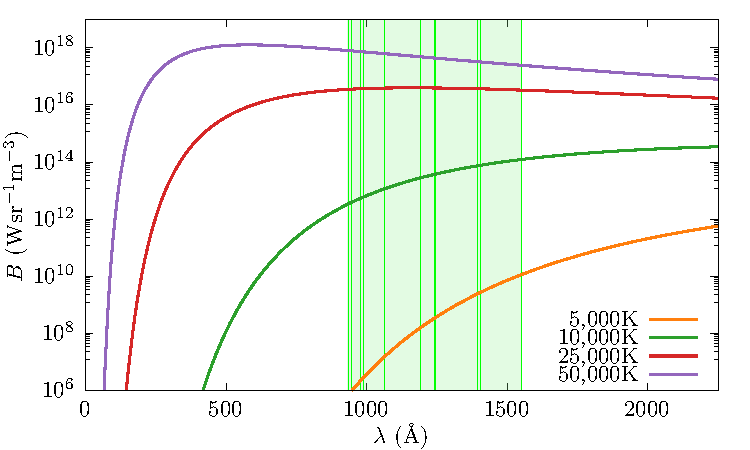
\includegraphics{assets/plancks-law/plancks-law.pdf}
  \caption[Planck's law radiance comparison with resonance lines]{Spectral radiance against wavelength for black body objects at various effective temperatures, $T_{\text{eff}}$, a series of wavelengths corresponding with important resonance lines in table 1 of \textcite{lucy_mass_1970} have been included. As temperature increases the spectral radiance at resonance line wavelengths dramatically increases, with a minimum of 6 orders of magnitude difference between the effective temperatures of a solar equivalent main sequence star and an O-type main sequence or Wolf-Rayet star.}
  \label{fig:planck-comp}
\end{figure}

% Need to briefly explain P-Cygni profiles as well

% Radiative line driving, this section may need to be beefed up

Early computations involving resonance lines from \textcite{lucy_mass_1970} provided a more reasonable mass loss rate calculation, but were still off by approximately two orders of magnitude.
Building off of the work by Lucy \& Solomon, a vital paper in the solidification of radiative lines as the main driving mechanism behind massive star outflows was produced by Castor, Abbott and Klein\footnote{Hereafter abbreviated as CAK.}.
The CAK formalism calculated reasonably close wind velocities, while being accurate to within a factor of 3 for mass loss rates \parencite{castor_radiation-driven_1975}.
Further work allowed for more accurate computations of the line driving effect, such as the mCAK prescription, the Sobolev approximation and the finite disk correction factor \parencite{pauldrachRadiationdrivenWindsHot1986}.

% Evolved OB stars, WR stars

As previously mentioned, evolved massive stars progress into a helium burning WR phase, at this point, mass loss rates due to radiative line driving are extreme, in the order of $10^{-5}$ \si{\solarmass\per\year}.
This outsized influence on the local medium can be seen in the production of ejecta nebula, such as M1-67 produced by WR 124 (figure \ref{fig:wr124}).

%//FIXME this is a placeholder, additionally how should I cite this?
\begin{figure}[h]
  \centering
  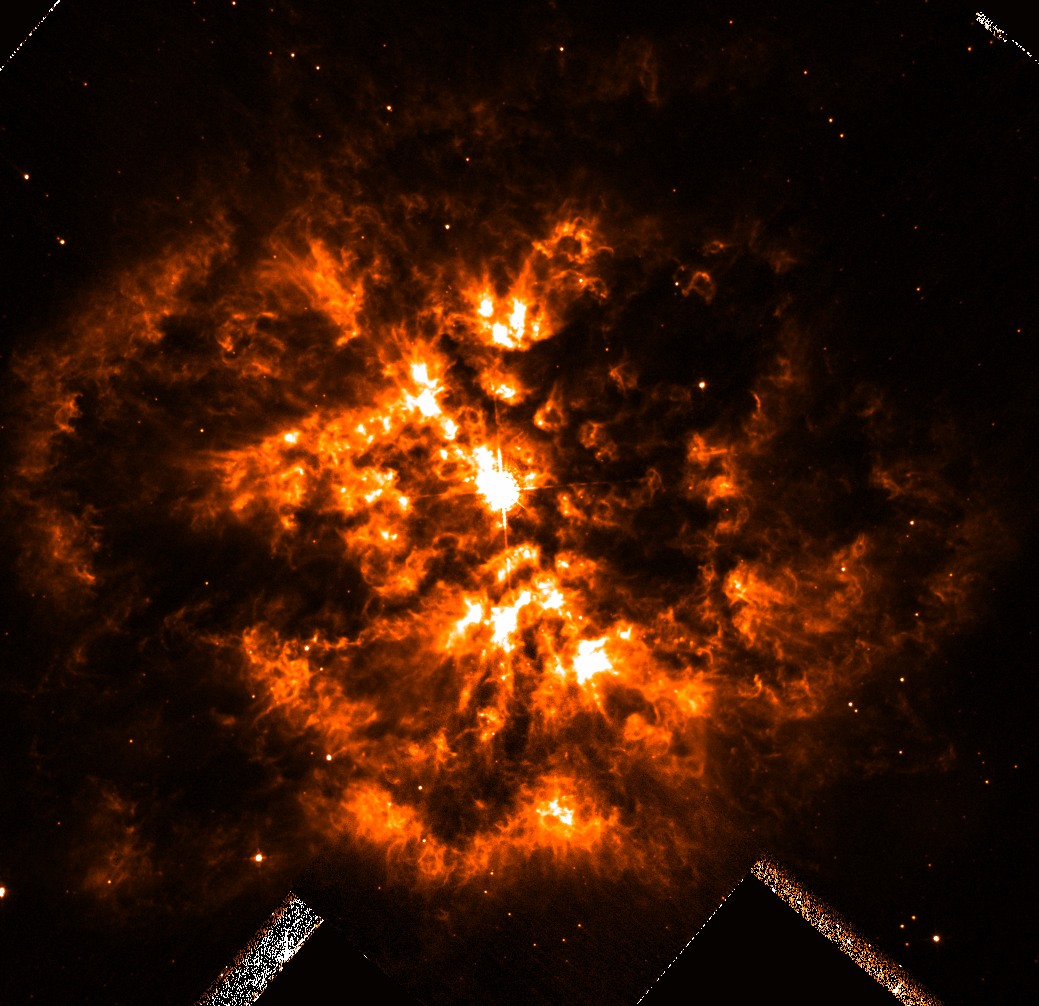
\includegraphics[width=4in]{assets/WR124.png}
  \caption[\textit{M1-67 nebula around WR 124 \parencite{2010ApJ...724L..90M}}]{Reduced Hubble WFPC2 data of the WN star WR 124, its extreme mass loss is currently producing the ejecta nebula M1-67 \parencite{2010ApJ...724L..90M}.}
  \label{fig:wr124}
\end{figure}

\begin{table}[h]
  \centering
  % \resizebox{\textwidth}{!}{%
  \begin{tabular}{cccc}
  \hline
  \multicolumn{1}{c}{Classification} & \multicolumn{1}{c}{$\dot M$} & \multicolumn{1}{c}{$v_\infty$} & \multicolumn{1}{c}{Mechanism} \\
  \multicolumn{1}{c}{}     & \multicolumn{1}{c}{\si{\solarmass\per\year}}         & \multicolumn{1}{c}{\si{\kilo\metre\per\second}}           & \multicolumn{1}{c}{}          \\ \hline
  Sun            & $10^{-14}$        & 400  & Thermal heating \\
  PMS & $10^{-4}-10^{-7}$ & 200-500 & Rotation \& magnetic fields \\
  Red Giant      & $10^{-7}-10^{-9}$ & 30   & Radiation pressure on dust grains        \\
  OB Star        & $10^{-7}-10^{-8}$ & 2500 & Radiation pressure \& line driving      \\
  Wolf-Rayet     & $10^{-5}$         & 1500 & Radiation pressure \& line driving       \\ \hline
  \end{tabular}%
  % }
  \caption[Stellar wind comparison]{Comparison of stellar winds emitted from various classification of star.}
  \label{tab:windcomp}
\end{table}

\begin{figure}
  \centering
  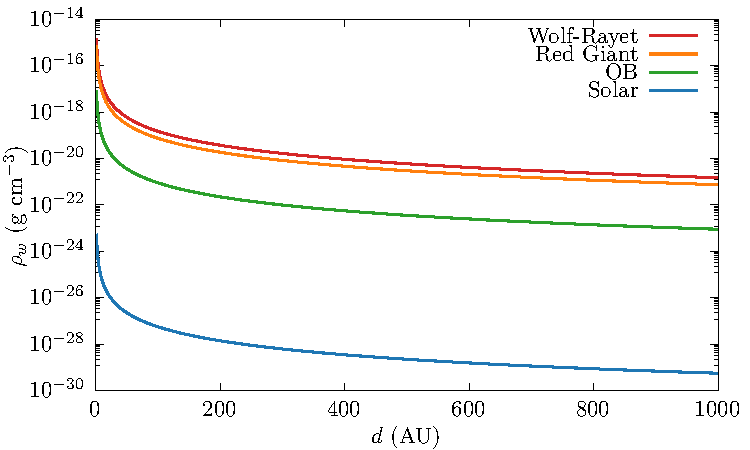
\includegraphics{assets/wind-comparison/wind-comp.pdf}
  \caption[$\rho_w$ comparison of main sequence winds]{Comparison of the densities of various main sequence winds using the parameters specified in table \ref{tab:windcomp}, wind densities are estimated using the smooth wind approximation described in equation \ref{eq:smoothwind}.}
  \label{fig:windrhocomp}
\end{figure}

\subsection{The CAK formalism}
\label{sec:cak}

\section{Interstellar Dust}
\label{sec:dust}

\subsection{The importance of interstellar dust}
\label{sec:dustimportance}

\subsection{Interstellar dust in massive star systems}
\label{sec:dustmassivestars}

\subsection{Radiation processes in interstellar dust}
\label{sec:dustcooling-background}

\section{Colliding Wind Binary Systems}
\label{sec:cwb}

Colliding Wind Binaries (abbreviated hereon to CWBs), in opposition to all known laws of astrophysical nomenclature, is a easy to understand term - it is a binary system where stellar winds from the member stars undergoing collision.
Unfortunately, the simplicity of the systems ends here, CWB systems are very poorly understood phenomena, due to a variety of factors that this section will discuss.

\subsection{History of CWB observation}

%History and classification, useful sources in Stevens & Pollock 1994 

Early observations beyond visual spectrum led to the discovery of many new astrophysical phenomena, one such discovery were extremely bright and variable thermal X-ray sources.
Many of these early galactic X-ray sources were found to be compact objects, and many more contained the characteristic spectral lines of a Wolf-Rayet star.
While single Wolf-Rayet stars are capable of producing X-ray emission, this is typically much dimmer than what was being observed 
\parencite{sewardXraysEtaCarinae1979}.

The existence of CWB systems were independently proposed by \textcite{prilutskii_x_1976} and \textcite{cherepashchukDetectabilityWolfRayetBinaries1976}, 
they proposed that significant and variable X-ray flux would result from the collision between two stellar winds, as these winds collide the gas becomes shocked and heated to temperatures on the order of \SI{1e8}{\kelvin}, hot enough to emit an appreciable quantity of X-rays.
The X-ray variability can also be explained as a result of the orbital properties of the systems, X-ray variability would result from the following effects:
% This may need to be expanded on or changed
\begin{itemize}
  \item Eccentricity in the orbits of the systems, leading to differing shock intensity and changing of the shock geometry, changing the fraction of the winds being shocked.
  \item Edge-on orbits resulting occlusion of X-rays by the stellar wind from each star. 
  \item Face-on orbits resulting in photospheric eclipses.
\end{itemize}

\noindent
Such effects could not be produced within a single star system \parencite{pittard_x-ray_1999}.
Further research by \textcite{pollockEinsteinViewWolfRayet1987} also found that single WR stars were typically faint, with the brightest X-ray emitting WR stars being confirmed to within massive binaries.
WR+OB systems were also found to be the brightest of such objects, while OB+OB binaries with significant X-ray flux were observed, these were typically less luminous.

% Early work categorising, using gamma 2 vel and V444Cyg

Early work was more concerned with X-ray observation, in particular the systems $\gamma^2$ Velorum and V444 Cygni, which were noted in particular as prototypical CWB systems by \textcite{prilutskii_x_1976}.
% Analysis pollock 1987 determined binary systems\cite{pollockEinsteinViewWolfRayet1987} 
Later, infrared observations of these systems found another, more curious attribute, a significant excess correlating to dust formation around these systems \parencite{williamsInfraredPhotometryLatetype1987}.
This will be discussed in more detail later in this section, but needless to say this phenomena is puzzling, as fragile grains of interstellar dust would not survive for long in the outflow of a WC star, due to the high wind temperatures and immense UV flux.
Because of this, dust growth was speculated, and later confirmed, to occur within the Wind Collision Region, the topic of the next section of this thesis.

\subsection{The Wind Collision Region}
\label{sec:wcr}

\begin{figure}
  \centering
  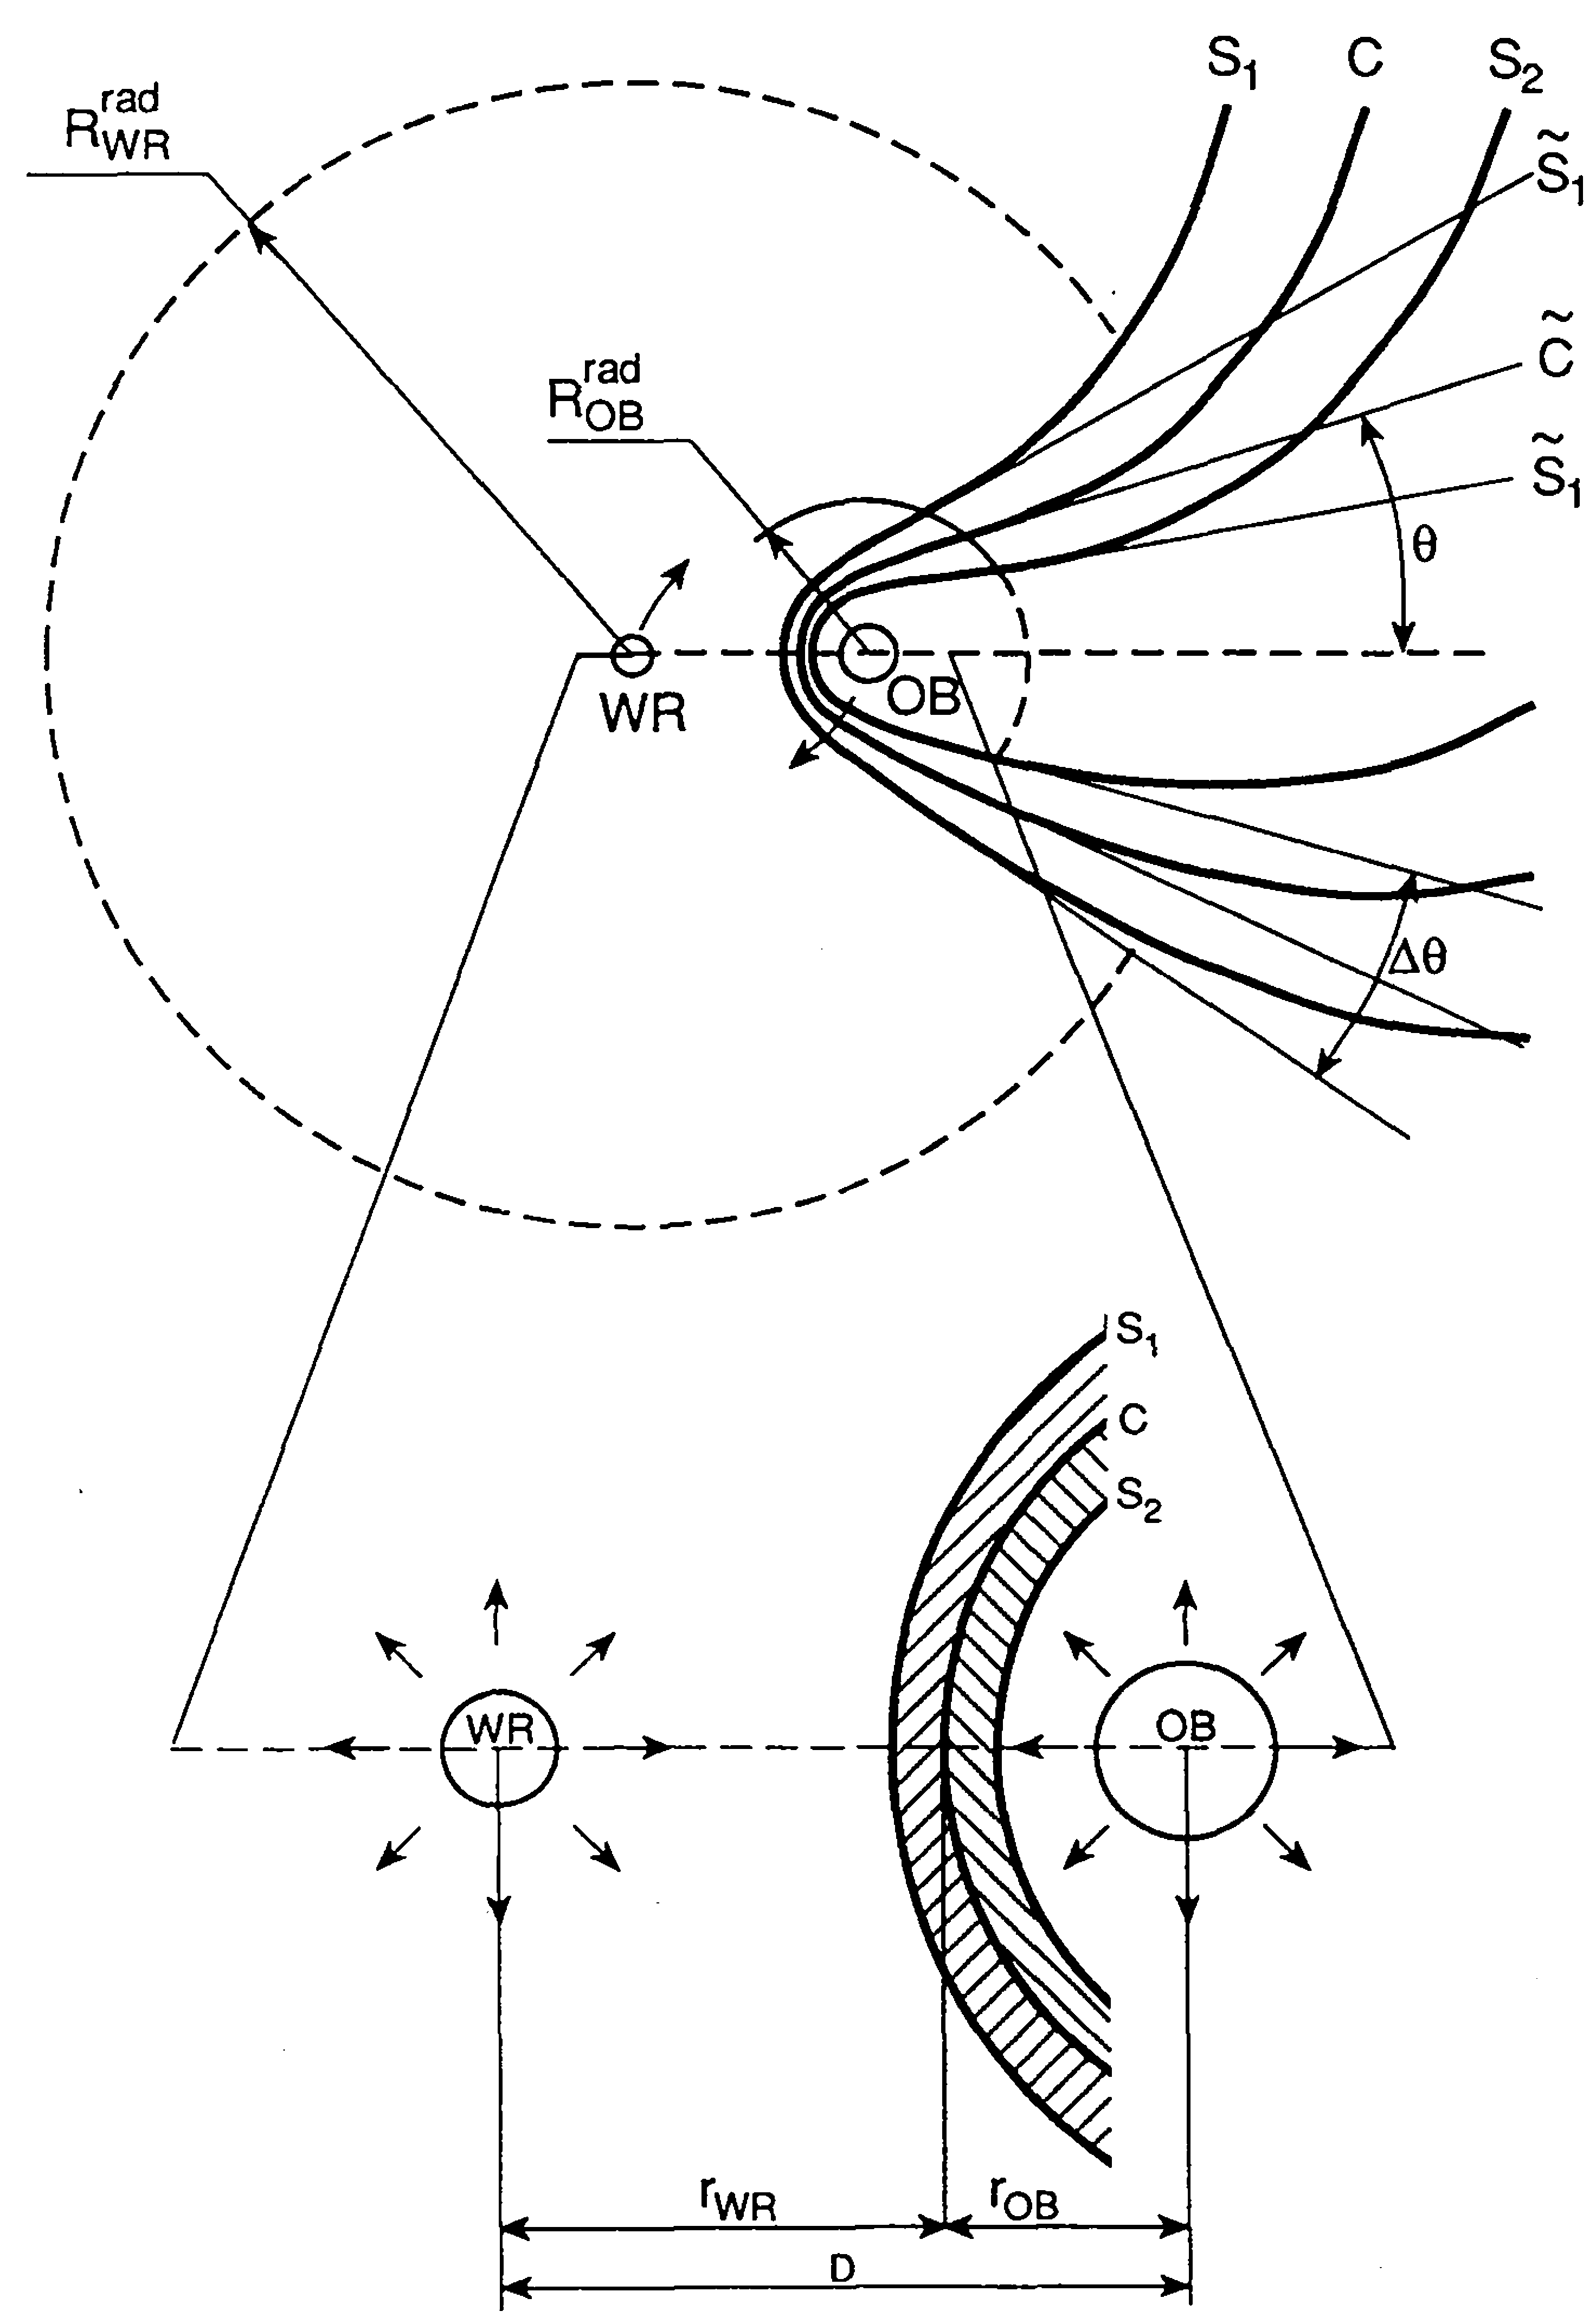
\includegraphics[width=3in]{assets/cwb-diagrams/eichler.png}
  \caption[\textit{A diagram of the Wind Collision Region \parencite{eichler_particle_1993}}]{A diagram of a typical Wind Collision Region inside a WR+OB CWB system. The $S_1$ and $S_2$ surfaces denote the shock waves from the primary and secondary winds respectively, and $C$ denotes the contact surface. The surfaces $\widetilde{S}_1$, $\widetilde{S}_2$ and $\widetilde{C}$ represent conic approximations of their corresponding surfaces at intermediate distances from the OB star. The region of stellar wind collision is hatched in the bottom diagram \parencite{eichler_particle_1993}.}
  \label{fig:wcr-diagram}
\end{figure}

\begin{figure}
  \centering
  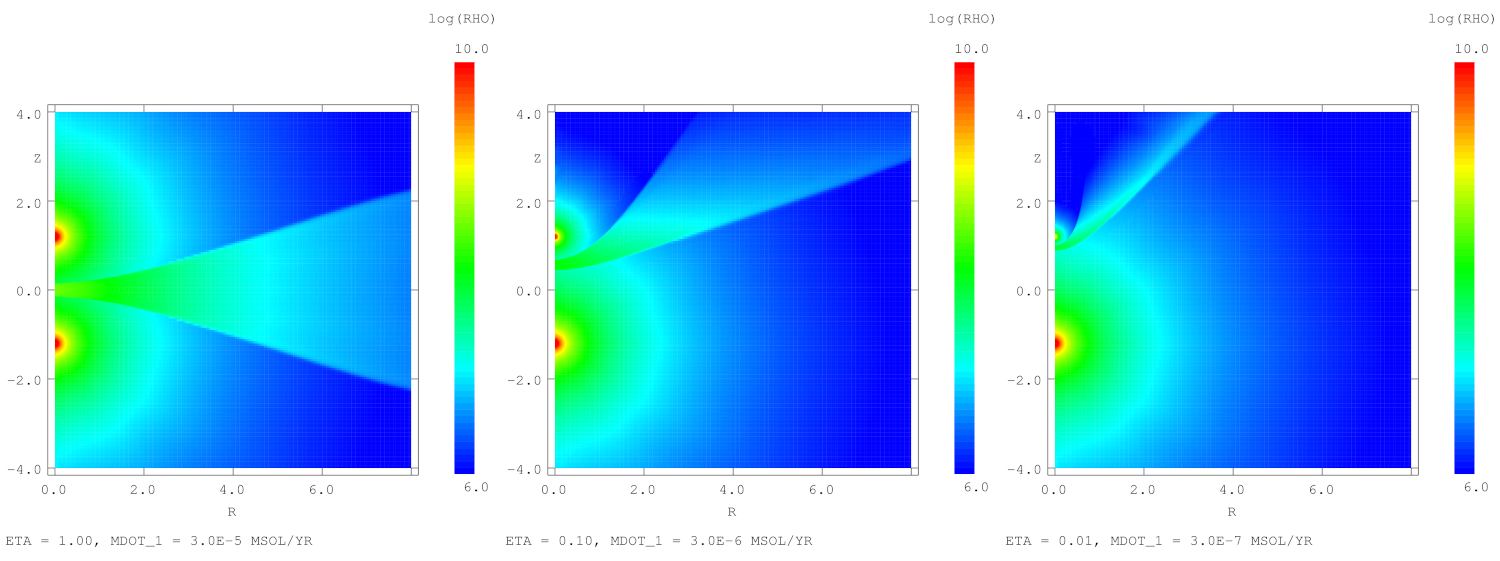
\includegraphics[width=6in]{assets/cwb-diagrams/eta.png}
  \caption[Comparison of wind momentum ratio, $\eta$, on WCR strtucture]{2D axisymmetric hydrodynamical simulations of CWB systems with wind momentum ratios of \num{1}, \num{0.1} and \num{0.001}. Momentum ratio is varied by changing the mass loss rate of the second star, $\dot{\text{M}}_2$. As $\eta$ decreases, the WCR begins to wrap itself around the secondary star.}
  \label{fig:wcr-eta}
\end{figure}

% What is this region
The Wind Collision Region (WCR) is the most violent and turbulent region of a CWB system, a region of high densities and even higher temperatures.
If the interacting stellar winds are dense as they begin to interact, a shocked region of plasma in excess of \SI{1e8}{\kelvin} is formed, the winds rapidly decelerate from hypersonic to subsonic, liberating an enormous amount of mechanical energy, on the order of \SI{1e3}{\solarluminosity}.
As previously discussed, this is the engine that drives the significant X-ray flux observed by astronomers in the 1970s, as well as other thermal and non-thermal emissions from the UV up to gamma rays \parencite{eichler_particle_1993,grimaldoProtonAccelerationColliding2019}.
As wind enters from either side of the wind collision region, it passes through a shock wave, and flows towards the centre of the wind collision region at the contact discontinuity, $C$ (figure \ref{fig:wcr-diagram}).
The wind behind the shock is driven by a combination of thermal pressure from the outflowing stellar wind, as well as the significant momentum the wind carried before being shocked \parencite{stevens_colliding_1992}.

The geometry of the WCR is influenced strongly by the wind parameters of both stars, the most important of which is the wind momentum ratio, or $\eta$, which we define as:

\begin{equation}
  \eta = \frac{\dot M_\text{OB} v^\infty_\text{OB}}{\dot M_\text{WR} v^\infty_\text{WR}},
\end{equation}

\noindent
where $\dot{\text{M}}_\text{WR}$ and $v^{\infty}_\text{WR}$ denotes the mass loss rate and wind terminal velocity of the primary, typically Wolf-Rayet star and $\dot{\text{M}}_\text{OB}$ and $v^{\infty}_\text{OB}$ denotes the mass loss rate and wind terminal velocity of the OB partner \parencite{usov_stellar_1991}.
A lower value of $\eta$ indicates a more unbalanced wind, with wind momentum ratio of \num{0.01} or lower being common for a typical WR+OB system.
Additionally, if $\eta = 1$, we observe a sheet of interacting plasma flowing away from the system perpendicular to the orbital plane.
In the case of a system where one stars momentum is significantly larger than the other, we observe the WCR extend and envelop the OB star, forming an approximately conical surface extending away from the Wolf-Rayet star (figure \ref{fig:wcr-eta}).


As the wind becomes more and more imbalanced, the contact discontinuity moves closer to the OB partner, this can be estimated with the equation:

\begin{equation}
  r_\text{WR} = \frac{1}{1+\eta^{1/2}} d_\text{sep} , ~~~ r_\text{OB} = \frac{\eta^{1/2}}{1+\eta^{1/2}} d_\text{sep} ,
\end{equation}

\noindent
where $r_{WR}$ is the distance from the WR star to the contact discontinuity, $r_\text{OB}$ is the distance from the OB star to the contact discontinuity and $d_\text{sep}$ is the orbital separation distance of the stars.

% Conic approximation


\begin{equation}
  \theta_c \simeq 2.1 \left(1 - \frac{\eta^{2/5}}{4}\right) \eta^{-1/3}, ~~ \text{for } 10^{-4} \leq \eta \leq 1, \label{eq:conic}
\end{equation}

% Wind shock factor, see Julians paper

% Analytical expressions of the opening angle for the shocks $S_1$ and $S_2$ have been provided by \textcite{pittardCollidingStellarWinds2018}.
% In this paper, a series of hydrodynamical simulations were performed with varying values of $\eta$, 
% The opening angle for $C$ was found to be consistent with the solution provided by \textcite{eichler_particle_1993}, while 

Work by \textcite{pittardCollidingStellarWinds2018} on determining the accuracy of opening angle expressions such as equation \ref{eq:conic} found that this approximation is accurate under the condition $\eta > 0.01$, but begins to diverge significantly if this condition is exceeded.
This was accomplished through a series of hydrodynamical simulations with different values for $\eta$, with the resultant opening angle calculated from the fully advected simulations.
This work goes on to derive analytical solutions to the opening angles of the conic approximations of $\widetilde{S}_1$ and $\widetilde{S}_2$, these solutions were found to be:

\begin{subequations}
  \begin{align}
    \theta_1 & = 2 \tan^{-1} \left(\eta^{1/3}\right) + \delta \theta , \\
    \theta_2 & = 0.658 \log_{10} \left(71.7 \eta \right) 
  \end{align}
\end{subequations}

\noindent
where $\delta \theta \approx \pi/9$.
From these estimations the fraction of each wind that is shocked, $f$, can be calculated:

\begin{subequations}
  \label{eq:windshockfraction}
  \begin{align}
    f_1 & = \frac{1 - \cos\left(\theta_1\right)}{2} , \\
    f_2 & = \frac{1 + \cos\left(\theta_2\right)}{2} .
  \end{align}
\end{subequations}

\noindent
\textcite{pittardCollidingStellarWinds2018} found that entirety of the secondary wind was shocked if $\eta \lesssim 0.014$, while in the typical wind momentum ratio regime typical of a WR+OB system ($0.001 \leq \eta \leq 0.01$), only $\approx 10\%$ of the WR wind is shocked (figure \ref{fig:wind-shock-factor}).
Whilst these analytical expressions are based on adiabatic simulations, and as such do not take into account the effect of a highly radiative WCR, they are still useful for setting an upper bound on dust production rates.

\begin{figure}
  \centering
  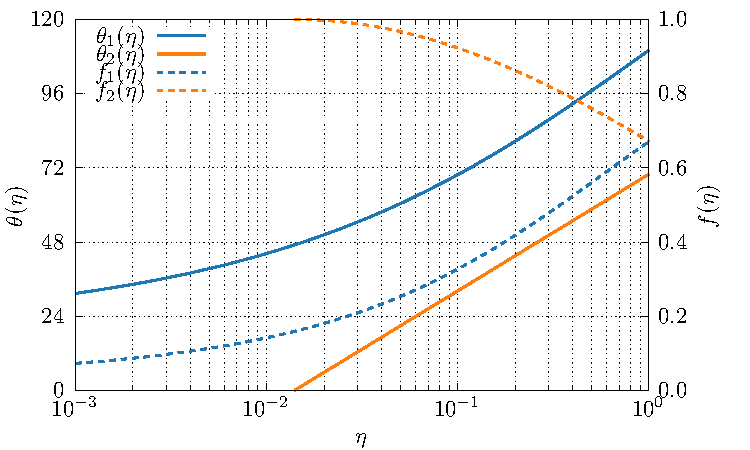
\includegraphics[]{assets/wind-shock-factor/shock-factor.pdf}
  \caption[Wind shock fraction, as a function of $\eta$]{Comparison of the opening angle of $\widetilde{S_1}$ and $\widetilde{S_2}$ as a function of $\eta$. The wind shock fraction, $f$, is also plotted. $\approx 10\%$ of the primary wind is shocked under typical WR+OB conditions, while the entire secondary wind is typically shocked.}
  \label{fig:wind-shock-factor}
\end{figure}

% Considerations due to stagnation point flow \cite{stevens_stagnation-point_1994}

%Detailed breakdown of Wind collision region

% Influence of orbital motion

\subsection{Cooling in the WCR}
\label{sec:wcrcooling}
%//TODO clean up this caption
%//TODO remove grid from plot
\begin{figure}[h]
  \centering
  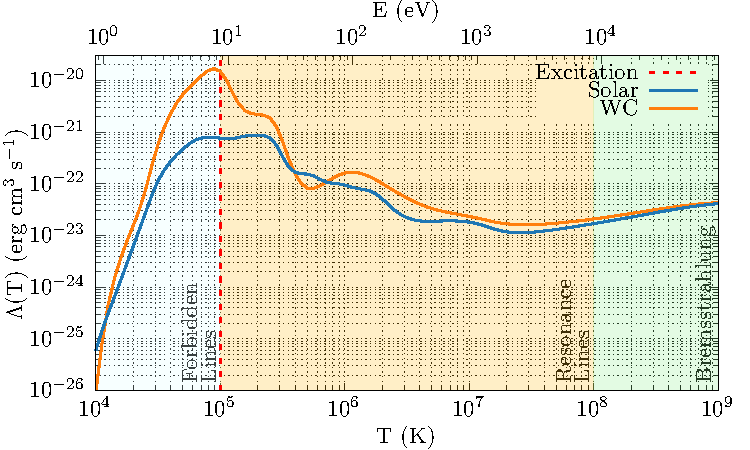
\includegraphics{assets/cooling-breakdown/cooling-curve-solar-withev.pdf}
  \caption[WC \& solar abundance plasma cooling curves]{Normalised plasma cooling rates as a function of temperature and thermal energy for solar abundance and WC abundance winds. The regions where forbidden line, resonance line and bremsstrahlung emission are dominant are highlighted, with H ionisation and recombination occuring between the forbidden and resonance line sections at $10^5$ \si{\kelvin}.}
  \label{fig:wcsolcooling}
\end{figure}

\begin{table}[h]
  \centering
  \begin{tabular}{lll}
  \\ \hline 
  \textbf{Temperature range} & \textbf{Dominant process} & \textbf{Spectral region} \\ \hline
  $\SI{5e3}{\kelvin} \lesssim T \lesssim \SI{1e5}{\kelvin} $ & Forbidden lines & IR, Optical \\
  $T \approx \SI{1e5}{\kelvin}$ & H excitation/ionisation & Optical, UV \\
  $\SI{5e3}{\kelvin} \lesssim T \lesssim \SI{1e5}{\kelvin} $ & Resonance lines & Far UV, soft X-ray \\
  $T \gtrsim \SI{1e8}{\kelvin} $ & Bremsstrahlung & Radio \\ \hline
  \end{tabular}
  \caption[Cooling processes at various temperature ranges]{Breakdown of dominant cooling processes at various temperature ranges from \cite{dysonPhysicsInterstellarMedium2021}, whilst H excitation/ionisation occurs over a very short temperature range, it is extremely influential, causing a global peak in the cooling rate at $\approx 10^5$ \si{\kelvin}. These temperature ranges are depicted in figure \ref{fig:wcsolcooling}.}
  \label{tab:coolprocess}
  \end{table}

% Radiative cooling, include graphs, mechanisms

Cooling due to radiation emission in a hot plasma can be broken down into a variety of processes that occur over series of temperature ranges.
Ions inside a plasma can become excited through collisions or photon absorption resulting in emission of photons as the ions de-excited. 

Mechanisms that are significant within the warm\footnote{See what I mean about the phrase ``warm''?} and hot gas phases include forbidden line emission, hydrogen excitation and ionisation, resonance lines and bremsstrahlung \parencite{dysonPhysicsInterstellarMedium2021}.
The influence of each mechanism waxes and wanes as temperature increases, with each mechanism dominant over a certain temperature range (table \ref{tab:coolprocess}).

% Section on forbidden line emission

The first mechanism to be discussed is forbidden line emission\footnote{Like many other phenomena discussed in this thesis, this too is a misnomer, while initially assumed to be prohibited under the contemporary understanding of atomic physics, it is in fact just astrophysicists jumping the gun again.}.
This process dominates the cooling process of cooler gas that is not fully ionised, where collisions with free electrons excite metallic elements within the gas, which de-excite through magnetic dipole and quadrupole fine structure state transitions.
This process dominates at these temperatures as the transition energies are significantly lower, on the order of \SI{1}{\electronvolt}, as the photon is also of a comparatively long wavelength, it can more easily escape from the surrounding gas.

% Section on ionisation/recombination

As the temperature increases there is a spike in the cooling rate of the gas as the hydrogen present begins to fully ionise, at this temperature a hydrogen ion and an electron may recombine, releasing a cascade of photons as the electron de-excites.

% Section on resonance line emission

As the plasma heats further resonance lines can

% Section on braking radiation

As the particle energy reaches the range of tens of \si{\kilo\electronvolt}, bremsstrahlung\footnote{Or braking radiation when you can't remember how to spell it.} becomes dominant (figure \ref{fig:wcsolcooling}). High velocity electrons are deflected by ions, emitting radiation in the process due to conservation of energy. 

% \parencite{1993ApJS...88..253S}
\parencite{schureNewRadiativeCooling2009}
\parencite{rybickiRadiativeProcessesAstrophysics2004}

%//TODO clean up this caption
%//FIXME use the new cooling code for this graph, early changes in ionisation fraction result in a different appearance from 1e4 to 1e6 kelvin!
\begin{figure}
  \centering
  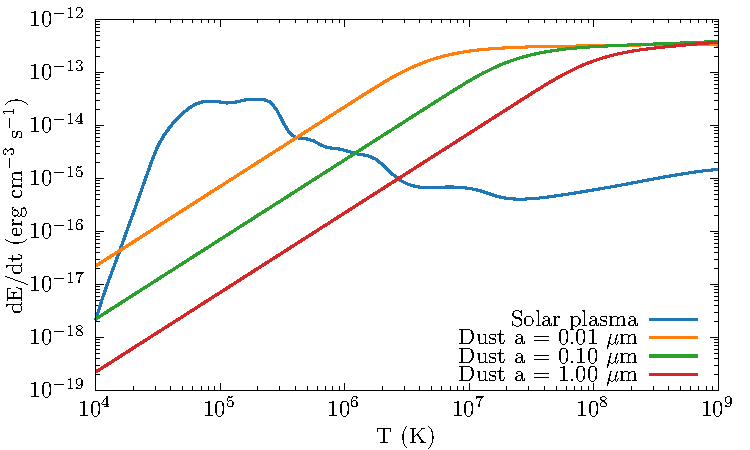
\includegraphics{assets/dust-plasma-cooling-comparison/cooling-comparison.pdf}
  \caption[Dust cooling vs. plasma cooling]{Comparison of plasma cooling to dust cooling with different grain sizes in a solar abundance gas, with a gas density of \SI{1e-20}{\gram\per\centi\metre\cubed} and a dust-to-gas mass ratio of 0.01.}
  \label{fig:dustplasmacomparison}
\end{figure}

% Needs to be spun off into a subsection

% Cooling parameter

\begin{subequations}
  \begin{align}
    \tau_\text{cool} & = \frac{k_B T_s}{4n_w \Lambda(T_s)} \label{eq:taucool} ,\\ 
    \tau_\text{esc}  & = \frac{d_\text{sep}}{c_s} \label{eq:tauesc} ,
  \end{align}
\end{subequations}

\begin{equation}
  \chi = \frac{\tau_\text{cool}}{\tau_\text{esc}} \approx \frac{v^4_{\infty,8} d_\text{sep,12}}{\dot M_{-7}} \label{eq:coolingparameter} ,
\end{equation}

% Dust cooling? Might need to move CWB dust formation up
The presence of dust within the immediate post-shock environment significantly increases the cooling rate.
Figure \ref{fig:dustplasmacomparison} compares rate of cooling due to dust emission of various types of grains to plasma cooling at solar abundances, 
As $\Lambda_g$ and $\Lambda_D$ are both proportional to $\rho_g^2$, dust cooling will dominate at high temperatures so long as there is sufficient amounts of dust.
%//TODO Lengthen paragraph, introduction to dust cooling

As dust grains collide with ionised gas and electrons, this imparts kinetic energy into the grains, heating them and causing them to emit infrared radiation. Assuming that there is a net accretion of ions and electrons onto the dust grains and the gas is optically thin in the infrared regime, energy is efficiently removed from the gas.
At particularly high temperatures this effect can dominate over high-temperature plasma cooling processes such as bremsstrahlung, as seen in figure \ref{fig:dustplasmacomparison}.
Figure \ref{fig:collisionalheatingcomparison} compares dust grain heating rates due to electron and ion collisional excitation in a solar abundance and WC abundance flow.
At lower temperatures the dust grain cooling rate is dominated by electron excitation, especially in the WC case as the ratio of free electrons to ions is significantly higher, as the WC flow is enriched by heavier elements.
However, as the grain temperature increases, collisional heating due to ions becomes more prevalent as the electrons are sufficiently energetic to pass through the grain without significant energy transfer; this is referred to as the electron transparency, $h_e$ \parencite{dwek_infrared_1981}.

\begin{figure}[h]
  \centering
  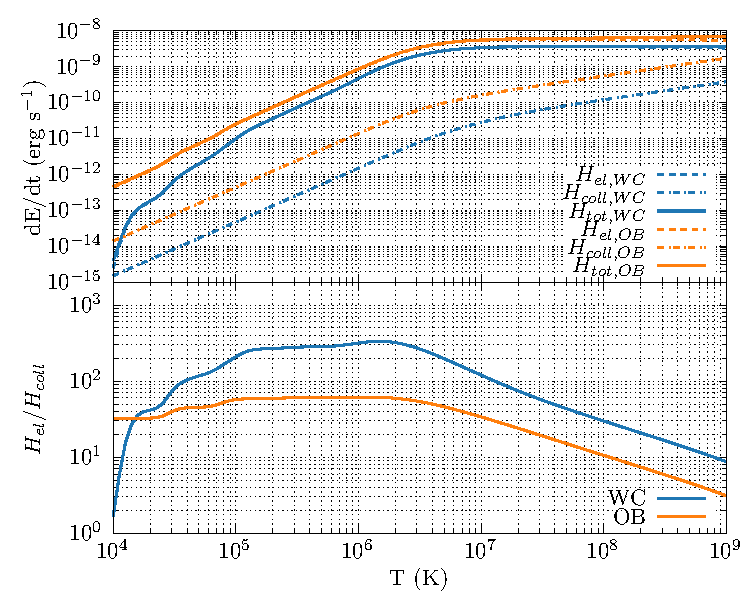
\includegraphics{assets/dust-electron-contribution/coll-el-comp.pdf}
  \caption[$H_{el}$ and $H_{coll}$ comparison]{Comparison of grain heating rate due to ion collisional excitation, $H_{coll}$, and electron excitation, $H_{el}$. The dust grain has a grain radius of \SI{5e-3}{\micro\metre} and is travelling through a gas with a density of $10^{-20}$ \si{\gram\per\centi\metre\cubed} with solar and WC abundances.}
  \label{fig:collisionalheatingcomparison}
\end{figure}

Work by \cite{dwek_infrared_1981} is used predominantly in this project to simulate cooling due to dust, a fast method for calculating the cooling rate due to dust was integrated into the numerical code for this project, which is elaborated on in section \ref{sec:dustcoolingmodel}.
% Finish and link to below paragraph

%Find citation for spitzer 1978

The heating rate of a dust grain due to collisions 

\begin{equation}
  \begin{split} 
      H_\text{coll} = & n \pi a^2 \langle Q(E,q,U) \rangle \\
      & \times \langle v (E-qU) f(a,E-qU) f(a,E-qU) \rangle \, \si{\erg\per\second}
  \end{split}
\end{equation}

%Explain constants
This can be simplified and expressed in the equation:

\begin{equation}
  \begin{split}
    H_\text{coll} & = \left(\frac{32}{\pi m}\right)^{1/2} n\pi a^2 (k_B T)^{3/2} h(a,T) \\
    & = \num{1.26e-19} \frac{n}{A^{1/2}} a^2 (\si{\micro\metre}) T^{3/2} h(a,T) \, \si{\erg\per\second}
  \end{split}
\end{equation}

% This part is very dry and is going to explain the equations more in depth
% Main source will be dwek 1981 appendix 2



% Instabilities due to cooling, might spin off into it's own appendix chapter?
% Theres a particular paper that covers this 
% Mainly need to discuss KH instabilities, and how they relate to cooling



\subsection{Dust formation in CWB systems}
\label{sec:cwbdust}

%Intro to dust formation in said systems
Despite the extremely violent conditions thus far described in CWB systems, these systems appear to be extremely prolific producers of interstellar dust.
Whilst single star WC systems can produce small amounts of dust in the form of amorphous carbon grains (though this could be observed to be extremely rare, pending the results of \textcite{medinaAreAllWCd2021}), binary systems have been observed to convert up to $10^{-3}$ of their wind masses from ionised carbon into amorphous carbon dust grains, this results in a typical dust production rate of $10^{-8} \, \si{\solarmass\per\year}$, on part with a typical Asymptotic Giant Branch (AGB) star.
This dust forming behaviour has only been observed in particularly energetic WC stars (predominantly WC9, with some WC7-8 examples), WN and WO systems have not been observed producing dust, this is most likely due to amorphous grains being significantly more chemically stable and resilient to effects such as sublimation and photoevaporation than water ice or silicate grains \parencite{salpeter_formation_1977,draineDestructionMechanismsInterstellar1979}.
Dust formation is also observed to form within the WCR, which can form quite beautiful pinwheel-shaped patterns, as dust streams away from the stars in the post-shock outflow.

\begin{table}[]
  \centering
  \begin{tabular}{ccccccc}
    & \multicolumn{2}{c}{Persistent} & \multicolumn{2}{c}{Variable} & \multicolumn{2}{c}{Episodic} \\ \cline{2-7} 
    & Total & Example & Total & Example & Total & Example \\ \hline
   WC4 & 1 & WR19 & 0 & --- & 0 & --- \\
   WC5 & 0 & --- & 0 & --- & 1 & WR47C \\
   WC6 & 1 & WR124-10 & 0 & --- & 0 & --- \\
   WC7 & 3 & WR102-22 & 0 & --- & 4 & WR140 \\
   WC8 & 6 & WR13 & 1 & WR48a & 3 & WR122-14 \\
   WC9 & 45 & WR104 & 6 & WR98a & 1 & WR75-11 \\ \hline
   Total & 56 &  & 7 &  & 9 &  \\ \hline
  \end{tabular}
  \caption[Numer of confirmed WCd systems]{Number of confirmed WCd systems with known spectral type and dust formation type from the Galactic Wolf Rayet Catalogue \parencite{rossloweSpatialDistributionGalactic2015}, systems with uncertain spectral types not included, while systems labelled ``d'' are included within the ``persistent'' category for their associated spectral type.}
  \label{tab:wc-summated-list}
\end{table}

% Rarity
Whilst beautiful, they are sadly an elusively rare beauty...
The Galactic Wolf Rayet Catalogue\footnote{The most recent version of this catalogue is available at \texttt{\href{http://pacrowther.staff.shef.ac.uk/WRcat}{http://pacrowther.staff.shef.ac.uk/WRcat}}} \parencite{rossloweSpatialDistributionGalactic2015} has a collection of 667\footnote{At time of time of writing, with the last update being August 2020.} known galactic WR stars, 106 of such stars are contained within a binary system, with 41 such binaries containing WC stars.
\textcite{rossloweSpatialDistributionGalactic2015} notes that there are a total of 42 confirmed WCd systems, approximately 35\% of all WC systems, though this value is somewhat out out date and includes single star systems.
A more up-to-date estimate performed for this thesis using the updated dataset estimates a total of 80 WCd systems, of which 72 have well-determined spectral subtypes (table \ref{tab:wc-summated-list}).
% Impact of systems 
\textcite{rossloweSpatialDistributionGalactic2015} goes on to estimate that out of an estimated total of 1900 galactic WR stars, approximately 300 of these stars are predicted to be dusty WC stars.
Whilst this is a far cry from the number of galactic AGB stars - of which carbon-rich AGBs outnumber WCd stars by approximately 3 orders of magnitude \parencite{ishiharaGalacticDistributionsCarbon2011} - these systems can still significantly impact the surrounding interstellar medium, with strong stellar feedback propagating large quantities of dust into the surrounding medium.

% Number of WCd systems, reasoning for only certain subtypes being dust forming
Table \ref{tab:wc-summated-list} contains an excerpt of the observed WCd systems with clearly defined spectral subtypes, most dust producing stars are either WC8 or WC9 subtypes, which are markedly cooler and less luminous than their WC4 counterparts.
This reduced luminosity is potentially the driving factor for dust formation in the system.
As WC8-9 systems have slower, cooler winds \parencite{niedzielskiKinematicalStructureWolfRayet2002}, they are more strongly influenced by post-shock cooling, allowing for greater dust formation within the WCR.
A small number of these systems have somewhat variable or episodic dust production cycles, such as WR98a and WR140, which are the two systems being observed within this thesis.
Furthermore, the bulk of WCd systems do appear to be in binary systems with a close periastron passage, in fact, this orbit itself appears to be a driving force behind how dust is produced in these systems, as we will later discuss.

%Theories as to why
A good starting point to understanding dust formation is to understand how the WCR can mitigate the mechanisms resulting in dust destruction, whilst aiding the processes involved in dust formation.
As previously discussed, dust can be destroyed through high-velocity collisions with grains, as well as evaporation through heating or ionising radiation.
These processes are mitigated through the cooling, as well as the high level of UV extinction due to the high density of the WCR.
Meanwhile, the dust production rate increases within high density regions, as collisions between dust grains and gas occur at a much higher rate.
The same can be said with dust grains, allowing for fast growth from gas and impinging ion accretion, and grain-grain collision as the number density of dust grains begins to increase.
The accumulation of these effects would be a very fast initial growth rate, which tapers off as the post-shock region diffuses and expands, resulting in a reduction in density.

% Role of instabilities
The presence of instabilities driven by cooling and other factors can lead to pockets of high density post-shock material, as high density drives dust formation, this can lead to ``clumps'' of highly dust-enriched post-shock stellar wind.
These clumps would have additional protection from UV photons, and would also be cooled enough for dust to form, thus, the driving hypothesis for this theory is that these are regions where the bulk of dust formation would occur.
% How to make lots of dust + reminder of aims of project.
As such, it is theorised in order to achieve a high rate of dust formation, a dense, highly radiative post-shock WCR must be formed, as cooling in the post-shock region is dependent on separation distance, wind velocity and mass loss rate, these parameters should first be explored, with the knowledge gleaned used to direct an analysis of observed systems such as WR140.

%Observational data Link to Crowther papers in particular, dust formations only around WC
% Discuss role of eccentricity
Eccentricity appears to play an important factor in the production of dust, highly eccentric systems can vary their dust production rates significantly.
Figure \ref{fig:periodicmags} shows the periodic change in mid-IR emission that can be explained as dust emission from small amorphous carbon grains, in the case of systems such as WR140 or WR125 dust production can be reduced to the point where associated emissions can drop by several magnitudes.
This relation is clearly periodic, with a peak in dust production production coinciding with the periastron passage of these systems.
This implies that dust production is dependent on orbital separation, which will influence the degree of cooling occurring within the WCR, it could potentially also alter the wind velocity on collision, which will also influence dust production in the same manner.
% Metastudy
Further analysis of available dust producing CWB systems suggests that \textit{all} WCd systems with circular orbits produce dust either persistently or with a degree of variability, while eccentric WCd systems are solely produce dust episodically.

\begin{figure}
  \centering
  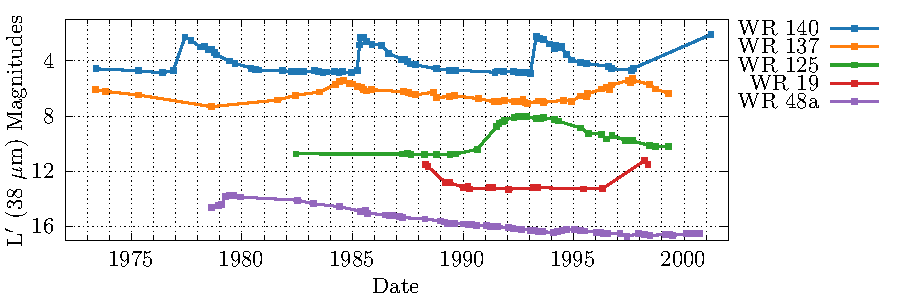
\includegraphics[]{assets/magnitudes/magnitudes.pdf}
  \caption[L$^\prime$ photometry of episodic dust making stars]{L$^\prime$ photometry for episodic dust making stars, data derived from \textcite{crowther_dust_2003}, and provided by PM Williams in private correspondence. WR 140 and WR 137 in particular have extremely predictable dust forming events which correspond to periastron passage in both systems.}
  \label{fig:periodicmags}
\end{figure}


\subsection{Important WCd systems}

The principle systems that are being observed in this thesis are the variable dust forming system, WR98a, and the episodic dust forming system WR140.
The archetypal continuous dust forming system WR104 was also proposed for simulation, but had to be cut due to time constraints, this system will also be discussed to provide a point of comparison between the two systems.

\begin{table}[h]
  \centering
  \begin{tabular}{cccccccc}
  \hline
  System & $\dot{\text M}_{\text{WR}}$ & $\dot{\text M}_{\text{OB}}$ & $v_{\text{WR}}^\infty$ & $v_{\text{OB}}^\infty$ & $\eta$ & $\chi_\text{min}$ & $\dot{\text M}_\text{D}$ \\
   & (\si{\solarmass\per\year}) & (\si{\solarmass\per\year}) & (\si{\km\per\second}) & (\si{\km\per\second}) & (AU) & & (\si{\solarmass\per\year}) \\ \hline
  WR98a & \num{5.0e-6} & \num{5.0e-8} & 900  & 2000 & 0.0222 & 0.7970 & $\left(6.10^{+1.77}_{-1.38}\right) \times 10^{-7}$ \\ 
  WR104 & \num{3.0e-5} & \num{6.0e-8} & 1220 & 2000 & 0.0033 & 0.2430 & $\left(4.39^{+1.27}_{-0.97}\right) \times 10^{-6}$ \\
  WR140 & \num{5.6e-5} & \num{1.6e-6} & 2895 & 3200 & 0.0314 & 2.6866 & $\left(8.11^{+4.83}_{-4.15}\right) \times 10^{-10}$ \\ \hline
  \end{tabular}
  \caption[Wind properties of systems considered for simulation]{Wind properties of systems considered for simulation in this thesis.}
  \label{tab:systems-wind-properties}
\end{table}

\begin{table}[h]
  \centering
  \begin{tabular}{ccccccc}
  \hline
  System & Period & Eccentricity & $M_{\text{WR}}$ & $M_{\text{OB}}$ & Periastron & Apastron \\
   & (d) & ($e$) & (\si{\solarmass}) & (\si{\solarmass}) & (AU) & (AU) \\ \hline
  WR98a & 556 & $\sim 0$ & 10.0 & 18.0 & 4.06 & 4.06 \\
  WR104 & 245 & 0.0600 & 10.0 & 20.0 & 2.20 & 2.48 \\
  WR140 & 2869 & 0.8993 & 10.31 & 29.27 & 1.53 & 26.9 \\ \hline
  \end{tabular}
  \caption[Orbital properties of systems considered for simulation]{Orbital properties of systems considered for simulation in this thesis.}
  \label{tab:systems-orbital-properties}
\end{table}

\subsubsection{WR98a}

\begin{figure}
  \centering
  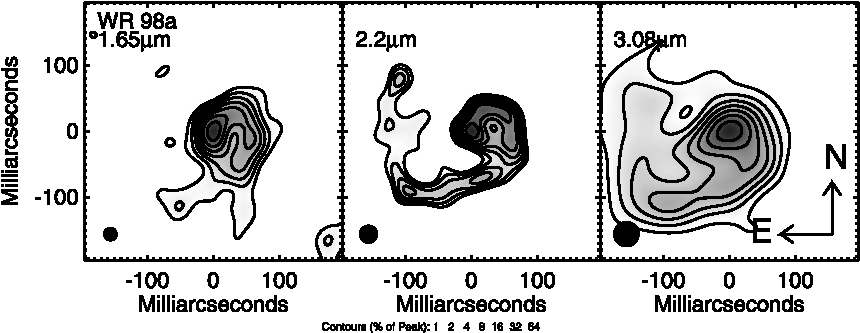
\includegraphics{assets/systems/wr98a-monnier2007.pdf}
  \caption[\textit{Multiwavelength image of WR98a \parencite{monnierKeckAperturemaskingExperiment2007}}]{Multiwavelength aperture synthesis images of WR98a taken on June \nth{24} 2000, at 1.65, 2.2, and \SI{3.08}{\micro\metre}. Plot sourced from \textcite{monnierKeckAperturemaskingExperiment2007}, the significant IR excess is a clear sign of ongoing dust production. The system also has a pronounced pinwheel structure most prominent at \SI{2.2}{\micro\metre}.}
\end{figure}

% Physical properties

WR98a is a  

% Historical observation 

% Hendrix paper dust formation monnier 2002 radio domain

% Questions as to orbit shape, approximately circular

% Ease of simulation, good starting point

% Parameter space exploration
Because of this relative ease of simulation and relatively slow wind velocity for both stars in the system, WR98a was chosen to be the baseline system for the research conducted in chapter \ref{chap:parameterspace}.

\subsubsection{WR140}

% Physical properties

% Historical observation
WR140 is significant in that it is the first system to be observed with episodic dust forming CWB properties, \textcite{williamsCondensationShellHD1978} notes a rapid brightening in the infrared, suggesting the formation of a new shell of dust around the system.
WR140 has undergone frequent observations, with spectroscopic data going back to 1972, and is perhaps the most well-observed episodic WCd system, for this it was immediately considered for 

% Eccentric orbit, variable dust formation

% Difficulty of simulation
As it is a highly eccentric system with a particularly long period orbit, a number of difficulties 

with the constraints of only having SMR available throughout this project, with AMR not currently being stable in this particular hydrodynamical code, 
% Snippet
As such, it was decided to only simulate the system as it undergoes closest approach, from $\phi = 0.95$ to $\phi = 1.10$, as a full orbit of the system would require AMR to undertake within the time constraints remaining in this project. 


\subsubsection{WR104}

\begin{figure}
  \centering
  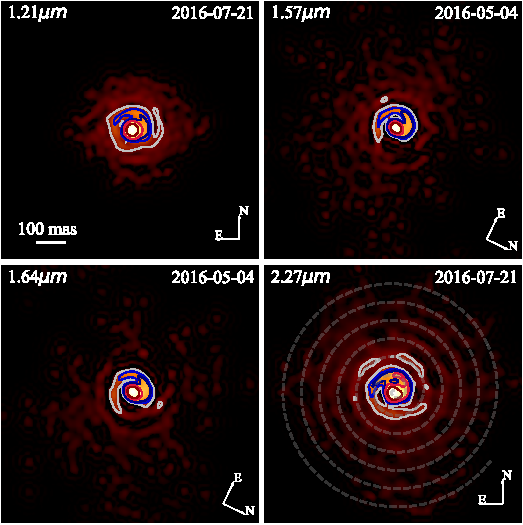
\includegraphics[]{assets/systems/soulain-2018-wr104.pdf}
  \caption[\textit{Spiral structure of WR104 \parencite{soulainSPHEREViewWolfRayet2018}}]{Deconvolution of J, H, K, and \SI{2.27}{\micro\metre} bands of WR104 sourced from \textcite{soulainSPHEREViewWolfRayet2018}. The spiral pattern and first revolution is visible in all images, in particular at \SI{2.27}{\micro\metre}.}
  \label{fig:soulain-wr104}
\end{figure}

% Physical properties
WR104 is an archetypal example of a continuous WCd system, it is a comparatively tight binary with a semi-major axis of \SI{2.34}{\au} and a period of $\sim 241$ days, the orbit is also relatively circular, with an eccentricity of $e = 0.06$ \parencite{lamberts_colliding_2012}.
The system consists of a WC9 star with a B0.5V partner \parencite{williamsSpectroscopyWC9WolfRayet2000}, this combination of a WC star and a comparatively weak B partner results in a severely imbalanced wind, with a momentum ratio of $0.003$, an order of magnitude lower than WR98a.
This imbalanced wind, combined with the tight orbit, results in an extremely strong WCR that is constantly churning out dust.
% Mass loss rate
Using radiative transfer models, \textcite{harries_three-dimensional_2004} calculated a dust production rate of \SI{8(1)e-7}{\solarmass\per\year}, corresponding to 2\% of the carbon mass loss rate of 
A more advanced model by \textcite{lauRevisitingImpactDust2020}, which is used to assess the dust formation rates of systems in this thesis, calculated the dust formation rate to be $\left(4.39^{+1.27}_{-0.97}\right) \times 10^{-6}\, \si{\solarmass\per\year}$.

% Why is it archetypal 

WR104 can be considered to be an ideal example of a continuous dust forming system, the system is relatively close, at a distance of \SI{2.5}{\kilo\parsec}, and is at an inclination that is almost face-on relative to Earth, at $i \lesssim 16^\circ$. 
As such, the pinwheel outflow from the system can be clearly resolved, with infrared excess due to dust clearly observed within the pinwheel structure (\textcite{soulainSPHEREViewWolfRayet2018}, see figure \ref{fig:soulain-wr104}).
Due to the systems parameters and well defined observable dusty pinwheel structure, along with prior observations and simulations of the system, it is an ideal candidate for simulation 

There are a number of reasons for this prodigious dust formation rate, as the systems orbit is comparatively close and circular with a very dense primary wind, the wind is expected to be highly radiative throughout the entire orbital period, this suggests a cool post-shock WCR that can continuously produce dust.
The estimated cooling parameter is more than an order of magnitude lower than the other systems considered for simulation, leading to a

% Why it wasn't assessed, difficulty of simulation, needed AMR
Unfortunately, despite being a very strong candidate for simulation, attempting to simulate the system proved to be exceptionally difficult.
% Many level simulation required for large-scale observation
The very close orbit of the system would mandate a very high simulation resolution, increasing the amount of compute time required to finish the simulation, only simulating a small region would prevent the pinwheel from being formed and observed, which we would have ideally wanted to include.
% Instability required running at very low Courant number
In addition the strong radiative cooling resulted in the simulation being very unstable unless the Courant number is exceedingly small, this also significantly increases compute time.
With a limited amount of compute resources as well as a limited amount of time, this stretched the feasibility of simulating this system.
% Physical effects, gayley
As the wind from the primary star is significantly stronger than its partners, WR104 has a much lower momentum ratio than the other systems being considered, as such, the WCR is situated much closer to the secondary star.
At closest approach, $r_\text{OB} \approx \SI{60}{\solarradius}$, which would require WR104 to be simulated at a much higher resolution, in turn demanding significantly more computational resources.
Physical effects, such as radiative inhibition and sudden braking may also significantly alter the wind velocity and post-shock environment, reducing the pre-shock primary wind velocity \textcite{gayley_sudden_1997}.
The pre-shock secondary wind velocity would also be influenced, due to insufficient acceleration from line driving before the winds collide.
As radiative line driving is not simulated these effects cannot be taken into account, and would have resulted in an inaccurate simulation of the system.
The effect of incomplete acceleration and sudden braking in highly wind-imbalanced systems is discussed more substantially in section \ref{sec:simassumptions}.
% Why it was discarded
With limited time remaining in the project, as well as the above factors, simulation work on WR104 was abandoned in favour of a parameter space search of a system with baseline properties similar to WR98a, as well as a limited simulation of WR140. 
Simulating this system however, is a particularly enticing avenue of future research.

\subsection{WR+WR systems}

Recently, two candidates of a theorised subset of CWB have been discovered - WR+WR systems, which have a \textit{second} Wolf-Rayet star as their partner, with a secondary wind around 3 orders of magnitude denser than a WR+OB system, this would of course result in a truly titanic wind collision.
These candidates are the recently discovered WR70-16 \parencite{callinghamAnisotropicWindsWolf2019}, and the previously discovered WR48a system \parencite{danksInfraredSpectroscopyInfrared1983}, which exhibits the spectroscopic lines of both a WC and WN system \parencite{williamsVariableDustEmission2019}.
These systems are predicted to be comparatively rare, even among CWB systems, this is largely due to unlikelihood that both stars in the system would be in their Wolf-Rayet phase at the same time.
Despite these systems having an enormous combined mass-loss rate, initial estimates of the dust production rates of both systems indicate that their dust conversion efficiencies are comparatively low compared to less energetic systems, and overall quite mundane dust production rates in general.
Whether this suppressed dust production rate is a common phenomena among WR+WR systems remains to be seen, as more systems would need to be discovered in order to determine this.

\subsubsection{WR70-16 (``Apep'') -- a recently discovered WR+WR system}

\begin{figure}
  \centering
  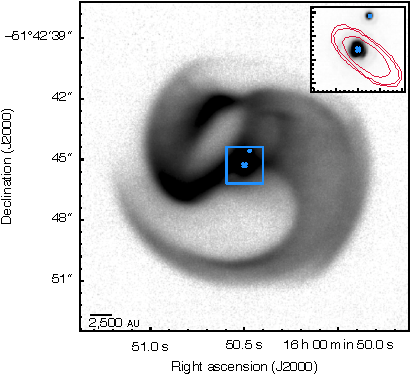
\includegraphics[]{assets/systems/apep-callingham-2019.pdf}
  \caption[\textit{VLT image of Apep \parencite{callinghamAnisotropicWindsWolf2019}}]{\textcite{callinghamAnisotropicWindsWolf2019}}
  \label{fig:apep-callingham}
\end{figure}

A potential avenue of research for this field is the simulation of WR+WR systems such as the recently discovered WR70-16 system (hereafter referred to as ``Apep''), this system was discovered due to the significant difference between the spectroscopically derived wind velocity of \SI{3400(200)}{\kilo\metre\per\second} and the observed expansion speed of \SI{570(70)}{\kilo\metre\per\second}  \parencite{callinghamAnisotropicWindsWolf2019}.
This inhibited wind velocity, far below any categorised WR wind velocity, suggests that much of the wind undergoes collision with the wind of a binary partner.
The extremely luminous non-thermal and infrared emission, suggested two extremely high mass loss rate stars within the system, as well as evidence for a third, distant partner in a loose trinary system \parencite{callinghamTwoWolfRayet2020}.
Spectroscopic analysis suggested that the central component of the Apep system consists of a nitrogen sequence WN4-6b and a carbon sequence WC8 star, with more more massive and luminous WN4-6b star kinematically dominating the system.
This discovery is very significant as it is the first galactic WR+WR system discovered, other systems have been identified, but are extragalactic in nature.

Further work by \textcite{hanExtremeCollidingwindSystem2020} has estimated the orbital parameters of Apep, finding that it is a highly eccentric system with a period of \SI{125(20)}{\year} and an eccentricity of \num{0.7(0.1)}, inclined at $\pm \ang{30} \pm \ang{5}$ towards Earth.
An initial estimate of the dust formation rate was made, finding a dust production rate of $\sim \SI{5e-7}{\solarmass\per\year}$, while observation of the surrounding dust shell suggests that it is a periodic dust forming system, which is sensible considering the systems high eccentricity.

The opening angle of the WCR was found to be very wide, at $\ang{125}\pm\ang{10}$, further suggesting the presence of two very high mass loss rate objects within the system, suggesting relatively balanced wind momenta for a CWB system.
Additional calculations by \textcite{marcoteAUscaleRadioImaging2021} estimated the systems wind momentum ratio to be $0.44\pm 0.08$, again in line with WR+WR hypothesis. 
Finally, pre-print work by \textcite{delpalacioNonthermalEmissionCollidingwind2021} finds a mass loss rate of \SI{4e-5}{\solarmass\per\year} for the WN star and \SI{2.9e-5}{\solarmass\per\year} for the WC star, which all but confirms the presence of a WR+WR binary at the heart of Apep.

With an estimated combined mass loss rate of \SI{6.9e-5}{\solarmass\per\year} we can estimate that the system has a dust conversion efficiency of 0.7\%;
whilst this system is therefore not a prodigious producer of dust this is most likely due to the extremely high wind terminal velocity and high separation distance, which would suggest a fairly smooth and adiabatic post-shock region. 
We can estimate the cooling parameter of the system to be $\sim 80$, based on angular separation from \textcite{hanExtremeCollidingwindSystem2020}, confirming that at present, the winds are adiabatic.
In order to estimate the closest approach of the system, and therefore the minimum cooling parameter an accurate measure of the stellar mass of both objects would need to be made, there is insufficient data for this at the time of writing.

\subsubsection{WR48a -- revisiting a WR+WR candidate}

% Why simulate it? And difficulties therein
WR+WR systems appear to be incredibly rare, with only a small number of extragalactic WN sequence examples in the LMC \parencite{shenarWolfRayetBinaries2019}, as well as an additional galactic WR+WR binary candidate, WR48a, \parencites(){zhekovMultiwavelengthViewDusty2014}{williamsVariableDustEmission2019}{zhekovChandraRevisitsWR2022}.
In the case of WR48a, its change in classification from a dust forming WC8 with an unknown partner to a WC8-WN8 is contemporaneous with the discovery and classification of Apep, though there is a distinct lack of recent observations of the system compared to the more recent WR+WR candidate.

\textcite{lauRevisitingImpactDust2020} calculated a dust formation rate for WR48a of $\left(8.46^{+3.48}_{-4.38}\right) \times 10^{-8} \, \si{\solarmass\per\year}$ with a dust conversion efficiency of $0.12\%$, markedly less than other systems with much less available material.
A future avenue of research would be to simulate these systems to understand why the dust formation rate is comparatively low, despite the readily available stellar material.
The main difficulty of simulating these systems is the lack of orbital parameters and accurate mass loss rates, as WR48a has insufficient data and Apep has only been recently discovered, there are currently too many unknown factors in order to build an adequate simulacrum of the systems\footnote{A lack of accurate orbital parameters is also an issue in devising simulations for more conventional WR+OB systems}.
Another difficulty is the large degree of orbital separation, high eccentricity and long orbital timescales required to simulate these systems.
The current limitations of the hydrodynamical code being used in this project render it difficult to simulate entire orbital passes of highly elliptical systems with long periods, if these issues are resolved in later versions of the hydro code however, this would present an interesting avenue of future research.
